\documentclass[a4paper,10pt,headlines=3.2]{scrartcl}
\usepackage{graphicx}           %Bilder

%\usepackage[T1]{fontenc}        %Umlaute
%\usepackage[latin1]{inputenc}   %Windows
%\usepackage[utf8x]{inputenc}	%Linux
\usepackage{ucs}

\usepackage[ngerman]{babel}     %Deutsche Sprache
\usepackage{amsmath}            %Math. Zeichen
\usepackage{pifont}             %Skalierbare Schriftart
\usepackage{array}
\usepackage{epsfig}             %Erweiterte Grafiken
\usepackage{makeidx}            %Stichwortverzeichnis
\usepackage[pdftex]{color} 

\newcommand{\changefont}[3]{
\fontfamily{#1} \fontseries{#2} \fontshape{#3} \selectfont}

\makeindex

\usepackage[automark]{scrpage2}
\usepackage[nosectionbib]{apacite}               %Zitieren

%\usepackage[colorlinks]{hyperref}%Hyperlinks

\usepackage{lmodern}
\usepackage{scrpage2}           %KOMA-Script
\usepackage{tipa}
\usepackage{qtree}
\usepackage{pgf}


\usepackage{remreset}			%Fussnoten global
\makeatletter
\@removefromreset{footnote}{chapter}
\makeatother 

\setcounter{tocdepth}{3}

%Kopfzeilen
\pagestyle{scrheadings}         %Seitenstil scrheadings verwenden

%\setlength{\textheight}{24cm}
%\setlength{\textwidth}{16cm}
%\setlength{\topmargin}{-2cm}
%\setlength{\oddsidemargin}{0cm}

% Groesse des Textbereiches in der Seite
\setlength{\textwidth}{16cm}
\setlength{\textheight}{22cm}
% Kopf- und Fusszeile, Hoehe und Abstand vom Text
\setlength{\headheight}{15pt}
\setlength{\headsep}{0.8cm}
% Linker Seiteneinzug
\setlength{\oddsidemargin}{2.5cm} \addtolength{\oddsidemargin}{-1in}
\setlength{\evensidemargin}{2.5cm} \addtolength{\evensidemargin}{-1in}
% Andere Groessen ausrechnen (vertikal zentrieren)
\setlength{\footskip}{\headsep}
\addtolength{\footskip}{\headheight}
\setlength{\topmargin}{\paperheight}
\addtolength{\topmargin}{-\textheight}
\addtolength{\topmargin}{-\headheight}
\addtolength{\topmargin}{-\headsep}
\addtolength{\topmargin}{-\footskip}
\addtolength{\topmargin}{-2in}
\addtolength{\topmargin}{-0.5\topmargin}

%Schriftart
\changefont{cmss}{m}{n}

%Abstand zur�cksetzen
\setlength{\headheight}{20pt}

\usepackage{listings} 
\lstset{numbers=left, numberstyle=\tiny, numbersep=5pt} \lstset{language=Java} 

\clearscrheadfoot
%\renewcommand{\headheight}{40pt} 
\ihead[]{Datenstrukturen und Algorithmen \\Fr�hlingssemester 2011 \\Institut f�r angewandte Mathematik} % - links
\ohead[asdasd]{�bung 9 \\Abgabetermin 5. Mai 2011 \\Adrianus Kleemans [07-111-693]} % - linke Kopfzeile 
\setheadsepline{.4pt} %Separate Linie im Kopf
\cfoot[\pagemark]{\pagemark} %- mittlere Fusszeile 

\begin{document}
\section*{Theoretische Aufgaben}
\subsection*{Aufgabe 1}
Zu zeigen: 
\begin{equation}
r_i(j) = 2^{n-j} 
\end{equation}
Induktionsanfang $j=n$,
\begin{equation}
r_j(n) = 2^{n-n} = 1 
\end{equation}
was �quivalent zur Gleichung 15.8 ist:
\begin{equation}
r_1(n)=r_2(n)=1 
\end{equation}
Induktionsschritt: $j=j-1$\\
Zu zeigen:
\begin{eqnarray}
r_i(j-1)=2^{n-(j-1)}\\
r_i(j-1)=r_1(j)+r_2(j)\\
=2^{n-j}+2^{n-j}\\
=2^{n-j+1} = 2^{n-(j-1)}
\end{eqnarray}
Zu zeigen:
\begin{equation}
\sum_{i=1}^{2}\cdot\sum_{j=1}^{2}\cdot r_i(j) = 2_{n+1}-2
\end{equation}
Indexverschiebung:
\begin{equation}
\sum_{j=1}^{n}\cdot 2^{n-j}=2^{n-i}+2^{n-2}+...+2^{n-n}=\sum_{j=0}^{n-1} 2^j = \frac{1-2^n}{1-2}=2^n-1
\end{equation}
Wird zu:
\begin{equation}
\sum_{i=1}^{2} \sum_{j=1}^{n} \cdot 2^{n-j}=\sum_{i=1}^{2}(2^n-1)=2^{n+1}-2
\end{equation}

\subsection*{Aufgabe 2}
Da die Teile vor oder nach jedem Arbeitsschritt vom einen aufs andere Band wechseln k�nnen, gibt es sehr viele M�glichkeiten. Viele dieser M�glichkeiten enthalten aber gleiche Teile, und will man den schnellsten Weg finden, kann in einem bestimmten Abschnitt eine optimale Teill�sung gefunden werden, der in der optimalen L�sung enthalten ist. Die Teill�sung ist aber abh�ngig von anderen Stationen (da Sie in direktem Austausch zu diesen steht) und teilt sich dieses Teilproblem mit einem andern Teilproblem.
\subsection*{Aufgabe 3}
Auf folgender Abbildung ist die funktionsweise eines LCS-Algorithmus zu sehen.
\begin{figure}[ht]
\centering
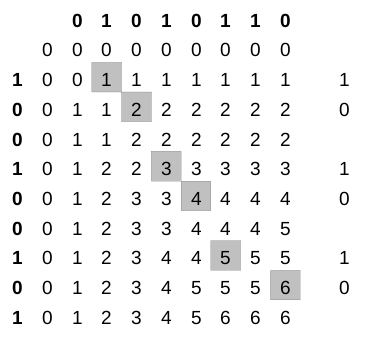
\includegraphics[height=6cm]{LCS}
\end{figure}
Eine m�gliche l�ngste gemeinsame Teilsequenz w�re demnach \texttt{101010}.

\newpage
\subsection*{Aufgabe 4}
Pseudocode f�r sichersten weg (bottom-up):
\lstset{frame=single}
\begin{lstlisting}[caption=Aufgabe 4]{Name}
//returns value of 'safest' way
int safestWay(int[][] area)
costs = new int[][] with same size as area
costs[0][0] = 0

for i = 0 to area.height - 1
   for j = 1 to area.width - 1
      if i == 0 
         costs[i][j] = costs[i][j-1] + area[i][j]
      else if j == 0
         costs[i][j] = costs[i-1][j] + area[i][j]
      else 
         costs[i][j] = min(costs[i][j-1], costs[i-1][j]) + area[i][j]
return costs[costs.height-1][costs.width-1]
\end{lstlisting}
Laufzeit des Algorithmus ist die Anzahl Felder, welche vorkommen, also $\Theta(h\cdot b)$, wenn h die H�he und b die Breite des Feldes repr�sentiert.

\begin{figure}[ht]
\centering
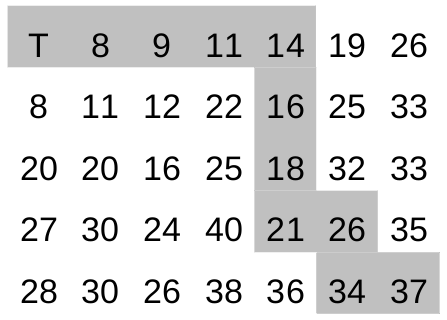
\includegraphics[height=5cm]{aufg4}
\end{figure}

Der Algorithmus ergibt die folgende L�sungstabelle. Startet man beim Endpunkt und vergleicht immer das obere und linke Feld und w�hlt dann das kleinere (dasjenige mit der tieferen Zahl) bis zum Anfang, so hat man den optimalen Weg gefunden.
Laufzeit ist die Anzahl Felder, welche durchlaufen werden m�ssen: $\Theta(h+b)$

\section*{Praktische Aufgaben}
\subsection*{Aufgabe 1 + 2}
Siehe Anhang \texttt{SeamCarving.java}.
\subsection*{Aufgabe 3}
Siehe Bildergalerie.
\newpage
\begin{figure}[h]
\begin{minipage}[t]{0.575\textwidth}
\centering
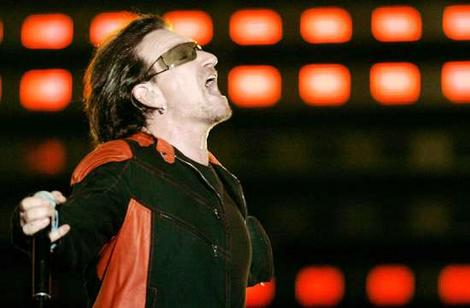
\includegraphics[height=5.5cm]{img/bono}
\vspace*{0.2cm}
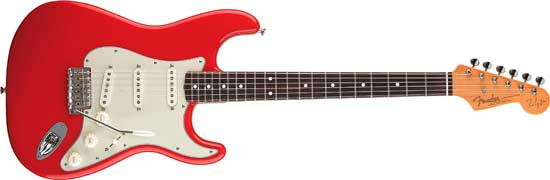
\includegraphics[height=2.8cm]{img/knopfler}
\vspace*{0.2cm}
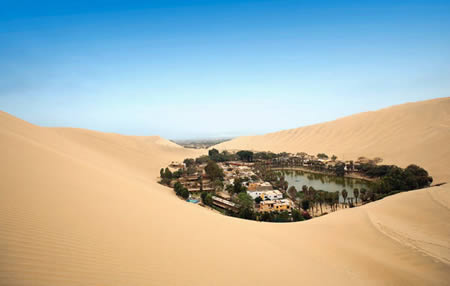
\includegraphics[height=5cm]{img/oase}
\vspace*{0.2cm}
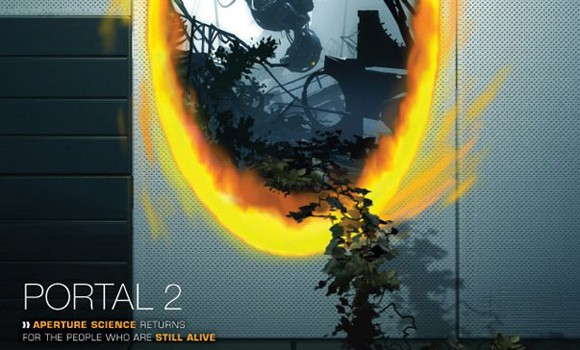
\includegraphics[height=4.8cm]{img/portal}
\end{minipage}
\hfill
\begin{minipage}[t]{0.375\textwidth}
\centering
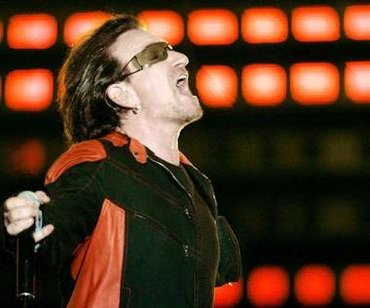
\includegraphics[height=5.5cm]{img/bono2}
\vspace*{0.2cm}
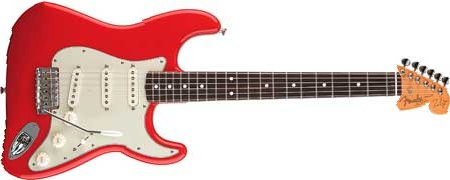
\includegraphics[height=2.8cm]{img/knopfler2}
\vspace*{0.2cm}
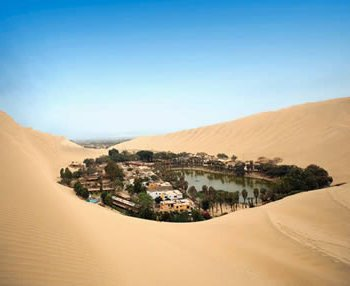
\includegraphics[height=5cm]{img/oase2}
\vspace*{0.2cm}
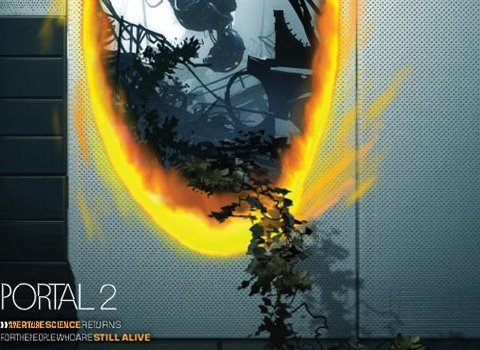
\includegraphics[height=4.8cm]{img/portal2}
\end{minipage}
\end{figure}

\end{document}